%!TeX encoding = UTF-8
%!TeX program = xelatex
\documentclass[notheorems, aspectratio=54]{beamer}
% aspectratio: 1610, 149, 54, 43(default), 32

\usepackage{latexsym}
\usepackage{amsmath,amssymb}
\usepackage{mathtools}
\usepackage{color,xcolor}
\usepackage{graphicx}
\usepackage{algorithm}
\usepackage{amsthm}
\usepackage{lmodern} % 解决 font warning
% \usepackage[UTF8]{ctex}
\usepackage{animate} % insert gif
\usepackage{lipsum} % To generate test text 
\usepackage{ulem} % 下划线,波浪线
\usepackage{autobreak}
\usepackage{multirow}
\usepackage{enumerate}
\usepackage{textcomp}
\usepackage{subfigure}




\usepackage{listings} % display code on slides; don't forget [fragile] option after \begin{frame}

% --------------- function-------------------------------
% tikx
\usepackage{framed}
\usepackage{tikz}
\usepackage{pgf}
\usetikzlibrary{calc,trees,positioning,arrows,chains,shapes.geometric,%
	decorations.pathreplacing,decorations.pathmorphing,shapes,%
	matrix,shapes.symbols}
\pgfmathsetseed{1} % To have predictable results
% Define a background layer, in which the parchment shape is drawn
\pgfdeclarelayer{background}
\pgfsetlayers{background,main}

% define styles for the normal border and the torn border
\tikzset{
	normal border/.style={orange!30!black!10, decorate, 
		decoration={random steps, segment length=2.5cm, amplitude=.7mm}},
	torn border/.style={orange!30!black!5, decorate, 
		decoration={random steps, segment length=.5cm, amplitude=1.7mm}}}

% Macro to draw the shape behind the text, when it fits completly in the
% page
\def\parchmentframe#1{
	\tikz{
		\node[inner sep=2em] (A) {#1};  % Draw the text of the node
		\begin{pgfonlayer}{background}  % Draw the shape behind
			\fill[normal border] 
			(A.south east) -- (A.south west) -- 
			(A.north west) -- (A.north east) -- cycle;
\end{pgfonlayer}}}

% Macro to draw the shape, when the text will continue in next page
\def\parchmentframetop#1{
	\tikz{
		\node[inner sep=2em] (A) {#1};    % Draw the text of the node
		\begin{pgfonlayer}{background}    
			\fill[normal border]              % Draw the ``complete shape'' behind
			(A.south east) -- (A.south west) -- 
			(A.north west) -- (A.north east) -- cycle;
			\fill[torn border]                % Add the torn lower border
			($(A.south east)-(0,.2)$) -- ($(A.south west)-(0,.2)$) -- 
			($(A.south west)+(0,.2)$) -- ($(A.south east)+(0,.2)$) -- cycle;
\end{pgfonlayer}}}

% Macro to draw the shape, when the text continues from previous page
\def\parchmentframebottom#1{
	\tikz{
		\node[inner sep=2em] (A) {#1};   % Draw the text of the node
		\begin{pgfonlayer}{background}   
			\fill[normal border]             % Draw the ``complete shape'' behind
			(A.south east) -- (A.south west) -- 
			(A.north west) -- (A.north east) -- cycle;
			\fill[torn border]               % Add the torn upper border
			($(A.north east)-(0,.2)$) -- ($(A.north west)-(0,.2)$) -- 
			($(A.north west)+(0,.2)$) -- ($(A.north east)+(0,.2)$) -- cycle;
\end{pgfonlayer}}}

% Macro to draw the shape, when both the text continues from previous page
% and it will continue in next page
\def\parchmentframemiddle#1{
	\tikz{
		\node[inner sep=2em] (A) {#1};   % Draw the text of the node
		\begin{pgfonlayer}{background}   
			\fill[normal border]             % Draw the ``complete shape'' behind
			(A.south east) -- (A.south west) -- 
			(A.north west) -- (A.north east) -- cycle;
			\fill[torn border]               % Add the torn lower border
			($(A.south east)-(0,.2)$) -- ($(A.south west)-(0,.2)$) -- 
			($(A.south west)+(0,.2)$) -- ($(A.south east)+(0,.2)$) -- cycle;
			\fill[torn border]               % Add the torn upper border
			($(A.north east)-(0,.2)$) -- ($(A.north west)-(0,.2)$) -- 
			($(A.north west)+(0,.2)$) -- ($(A.north east)+(0,.2)$) -- cycle;
\end{pgfonlayer}}}

% Define the environment which puts the frame
% In this case, the environment also accepts an argument with an optional
% title (which defaults to ``Example'', which is typeset in a box overlaid
% on the top border
\newenvironment{parchment}[1][Example]{%
	\def\FrameCommand{\parchmentframe}%
	\def\FirstFrameCommand{\parchmentframetop}%
	\def\LastFrameCommand{\parchmentframebottom}%
	\def\MidFrameCommand{\parchmentframemiddle}%
	\vskip\baselineskip
	\MakeFramed {\FrameRestore}
	\noindent\tikz\node[inner sep=1ex, draw=black!20,fill=white, 
	anchor=west, overlay] at (0em, 2em) {\sffamily#1};\par}%
{\endMakeFramed}

% ----------------------------------------------

\mode<presentation>{
	\usetheme{CambridgeUS}
	% Boadilla CambridgeUS
	% default Antibes Berlin Copenhagen
	% Madrid Montpelier Ilmenau Malmoe
	% Berkeley Singapore Warsaw
	\usecolortheme{beaver}
	% beetle, beaver, orchid, whale, dolphin
	\useoutertheme{infolines}
	% infolines miniframes shadow sidebar smoothbars smoothtree split tree
	\useinnertheme{circles}
	% circles, rectanges, rounded, inmargin
}
% 设置 block 颜色
\setbeamercolor{block title}{bg=red!30,fg=white}

\newcommand{\reditem}[1]{\setbeamercolor{item}{fg=red}\item #1}

% 缩放公式大小
\newcommand*{\Scale}[2][4]{\scalebox{#1}{\ensuremath{#2}}}

% 解决 font warning
\renewcommand\textbullet{\ensuremath{\bullet}}

% ---------------------------------------------------------------------
% flow chart
\tikzset{
	>=stealth',
	punktchain/.style={
		rectangle, 
		rounded corners, 
		% fill=black!10,
		draw=white, very thick,
		text width=6em,
		minimum height=2em, 
		text centered, 
		on chain
	},
	largepunktchain/.style={
		rectangle,
		rounded corners,
		draw=white, very thick,
		text width=10em,
		minimum height=2em,
		on chain
	},
	line/.style={draw, thick, <-},
	element/.style={
		tape,
		top color=white,
		bottom color=blue!50!black!60!,
		minimum width=6em,
		draw=blue!40!black!90, very thick,
		text width=6em, 
		minimum height=2em, 
		text centered, 
		on chain
	},
	every join/.style={->, thick,shorten >=1pt},
	decoration={brace},
	tuborg/.style={decorate},
	tubnode/.style={midway, right=2pt},
	font={\fontsize{10pt}{12}\selectfont},
}
% ---------------------------------------------------------------------

% code setting
\lstset{
	language=C++,
	basicstyle=\ttfamily\footnotesize,
	keywordstyle=\color{red},
	breaklines=true,
	xleftmargin=2em,
	numbers=left,
	numberstyle=\color[RGB]{222,155,81},
	frame=leftline,
	tabsize=4,
	breakatwhitespace=false,
	showspaces=false,               
	showstringspaces=false,
	showtabs=false,
	morekeywords={Str, Num, List},
}

% ---------------------------------------------------------------------

%% preamble
\title[Suggestions for Retaurants]{\LARGE\textbf{{How to Improve Your Restaurant?}}}
% \subtitle{The subtitle}
\author[L.Du, L.Ma, W.Xie]{Lize Du, Linquan Ma, Wenjia Xie}
\institute{STAT 628}

% -------------------------------------------------------------

\begin{document}
	
	%% title frame
	\begin{frame}
	\titlepage
\end{frame}

%% normal frame
\begin{frame}
\frametitle{Outline}
\begin{itemize}
	\item[\textcolor{darkred}{\textbullet}] Data cleaning
	\vspace{2ex}
	\item[\textcolor{darkred}{\textbullet}] Deal with Review Dataset
		\vspace{2ex}
	\item[\textcolor{darkred}{\textbullet}] Suggestions for Restaurants
	\begin{itemize}
		\item[\textcolor{darkred}{\checkmark}] Some Informative Words	
		\item[\textcolor{darkred}{\checkmark}] Word Clouds
		\item[\textcolor{darkred}{\checkmark}] Geography
	\end{itemize}
	\vspace{2ex}
	\item[\textcolor{darkred}{\textbullet}] Future Work
\end{itemize}
\end{frame}

\begin{frame}
\frametitle{Data Cleaning: Business Dataset}
\begin{figure}[H]
	\centering
	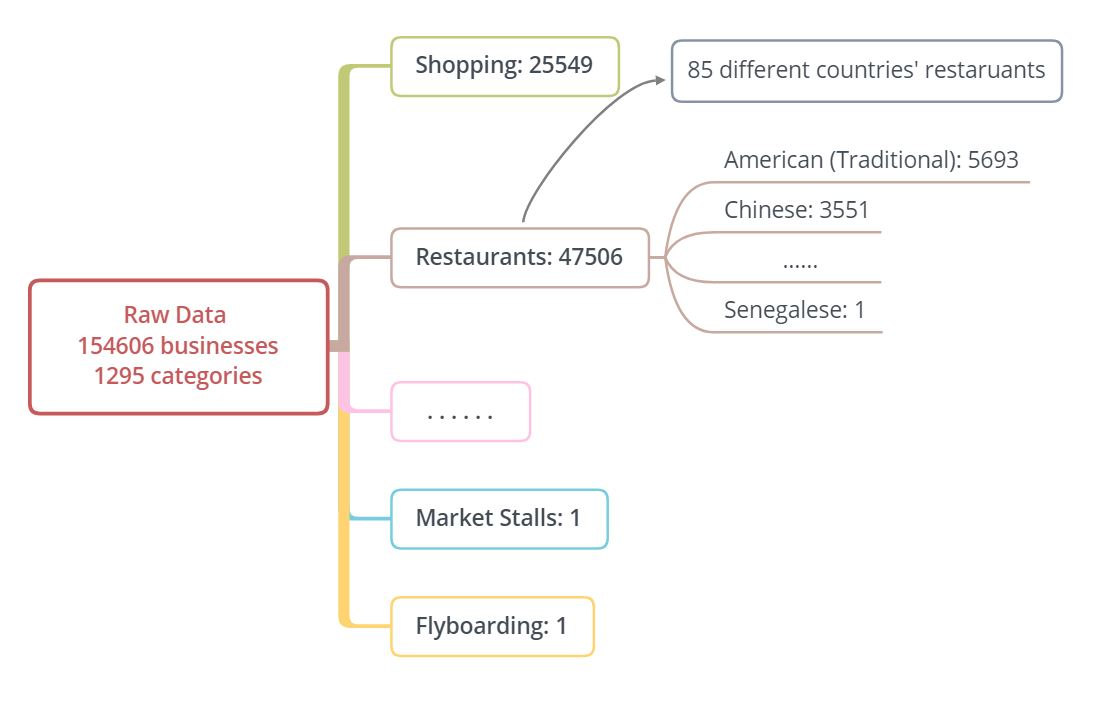
\includegraphics[width=4.6in]{dataclean_business.jpg}
\end{figure}
\end{frame}

\begin{frame}
\frametitle{Data Cleaning: Review}
\begin{itemize}
	\item[\textcolor{darkred}{\textbullet}] Stopwords use $nltk.stopwords.words$ except:
	\begin{itemize}
		\item[\textcolor{darkred}{1}] Third person pronoun: he, she, it, they, their
		\item[\textcolor{darkred}{2}] Adverb of degree: few, most, more...
		\item[\textcolor{darkred}{3}] Negative: don’t, didn’t, doesn’t aren’t...		
	\end{itemize}
    \item[\textcolor{darkred}{\textbullet}] Pattern matching: words, abbreviation, [a-zA-Z]-[a-zA-Z], … , ?, ! 
    \item[\textcolor{darkred}{\textbullet}] Substitute: he's$\rightarrow$he is, n'/n't$\rightarrow$not, 'd$\rightarrow$would...
    \item[\textcolor{darkred}{\textbullet}] Delete: noun’s, number+th/st/nd/rd;
    \item[\textcolor{darkred}{\textbullet}] Change to lower case;
    \item[\textcolor{darkred}{\textbullet}] Tokenize using regular expression;
    \item[\textcolor{darkred}{\textbullet}] Add \_neg to the words between not/never and the first punctuation;
    \item[\textcolor{darkred}{\textbullet}] Use porter stemmer to do stem extracting, such as amazing$\rightarrow$amaz;
    \item[\textcolor{darkred}{\textbullet}] Use wordnet lemmatizer to lemmstize the verb to a normal form, such as loving$\rightarrow$love
\end{itemize}
\end{frame}

\begin{frame}
\frametitle{Deal with Review Dataset}
\ \ \ \ All review: 3.43 GB

\ \ \ \ American restaurants' review: 503 MB; 845,941 rows 

\ \ \ \ \ \ \ \ \ ($grep$ command in bash)

\vspace{2ex}
\ \ \ \ Dictionary size: 245,344 words

\vspace{2ex}
\ \ \ \ 1. For the first part, just focus on some top words based on 

\ \ \ \ \ \ \ \  frequency, so only contains the most frequent 461 words.

\ \ \ \ 2. Count every word’s frequency in every star (even if it appears 

\ \ \ \ \ \ \ \ many times in one review, we just focus on if it appears)

\ \ \ \ 3. Use \color{darkred}{information gain} \color{black}of each word to rank them.

\end{frame}

\begin{frame}
\frametitle{How to Define Information Gain?}
$$\mathrm{Information\ gain} = H(Y) - H(Y|X)$$

where $Y$ denotes class (star level), $X$ is feature (word).

\ \ \ \ For example, the proportion of each star in whole dataset is $P_i$, i = 1, 2, 3, 4, 5. 
$$H(Y)=-\sum_{i=1}^{5}P_i log_2 P_i$$
\ \ \ \ if we specify $x$ as "good",
$$H(Y|X)=\sum_{i=1}^{2}P(X=x_i)(-\sum_{j=1}^{5}P_{ij} log_2 P_{ij})$$
where $x_i$ = 0, 1 (1 denotes review contains "good"), $p_{ij}$ is proportion of star j when $X=x_i$
\end{frame}

\begin{frame}
\frametitle{Informative Words (Positive)}
\begin{figure}[H]
	\centering
	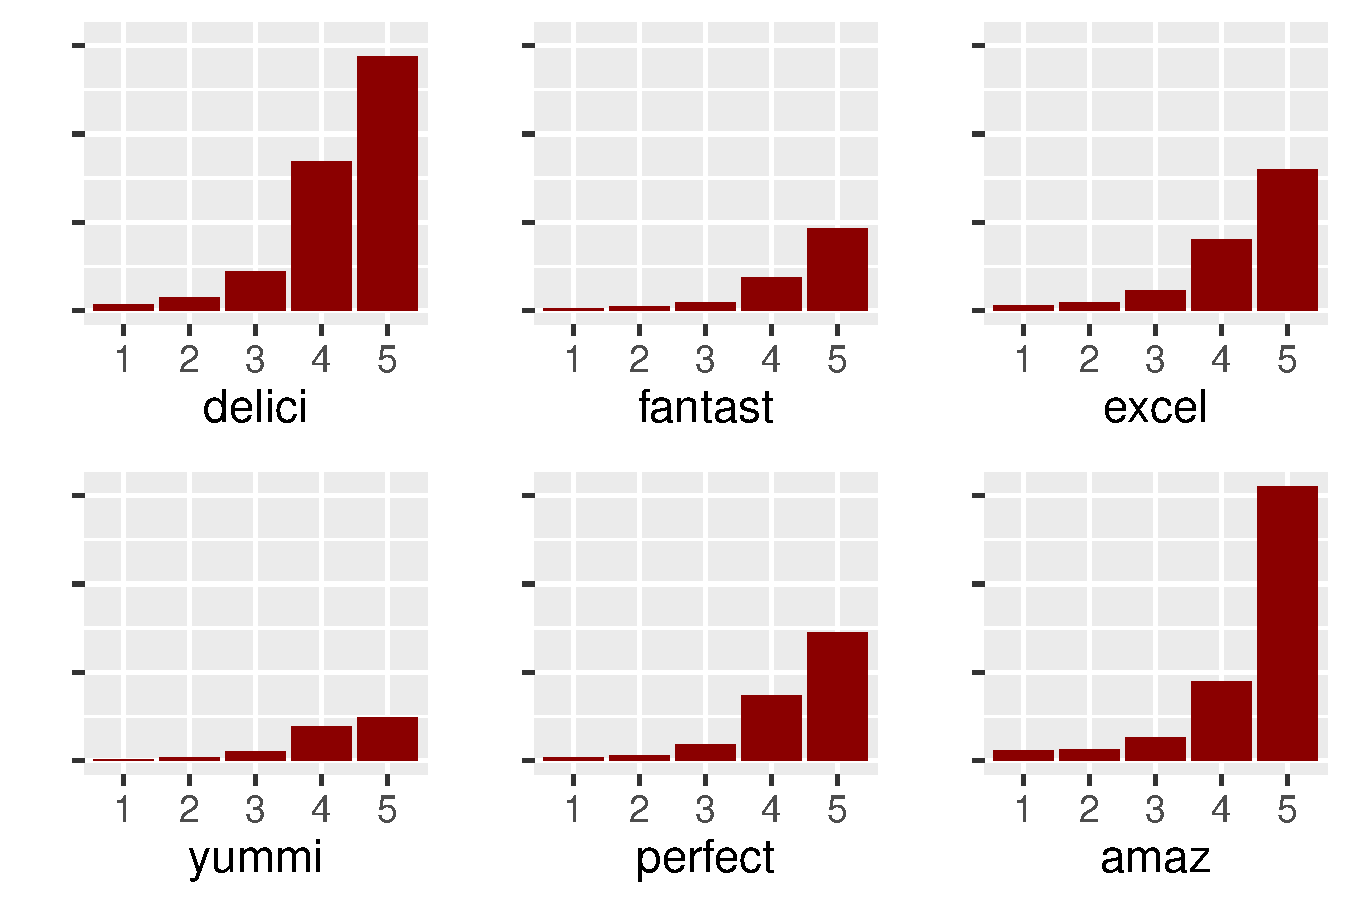
\includegraphics[width=4.6in]{positive.pdf}
\end{figure}
\end{frame}

\begin{frame}
\frametitle{Informative Words (Negative)}
\begin{figure}[H]
	\centering
	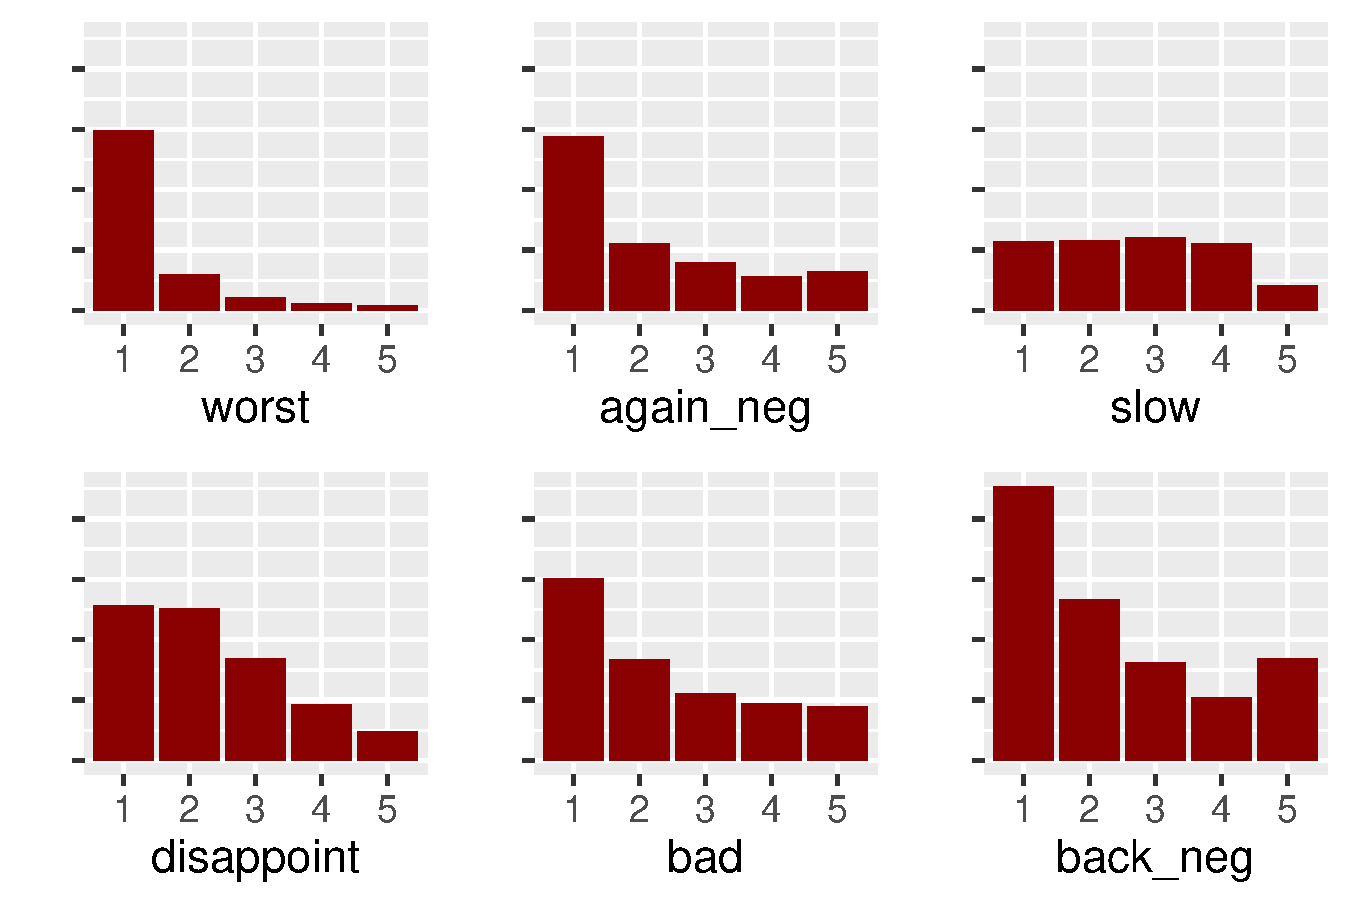
\includegraphics[width=4.6in]{negative.pdf}
\end{figure}
\end{frame}

\begin{frame}
\frametitle{Punctuation}
\begin{figure}[H]
	\centering
	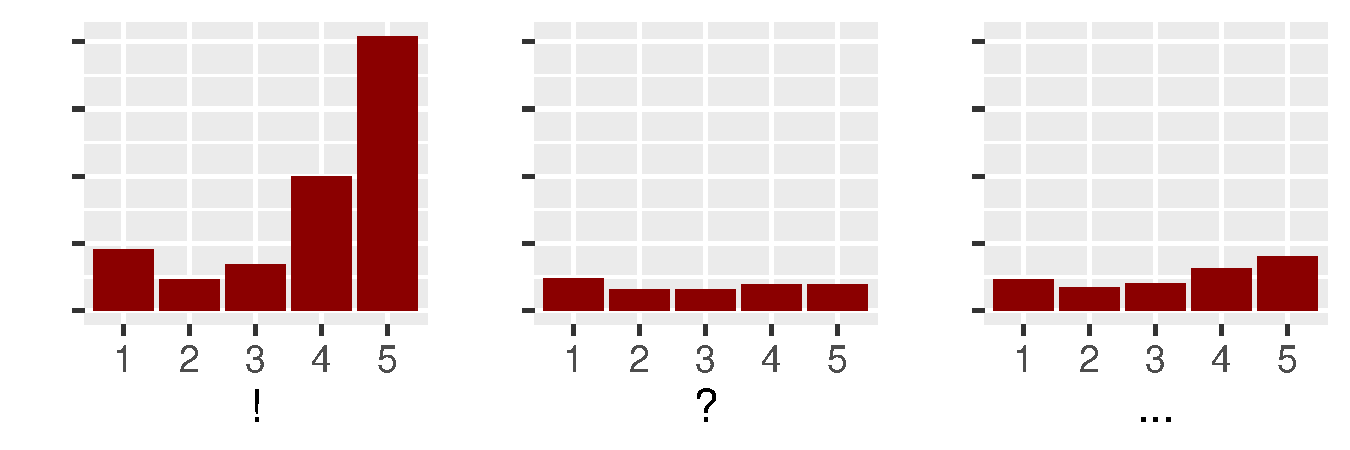
\includegraphics[width=4.6in]{punctuation.pdf}
\end{figure}
\end{frame}

\begin{frame}
\frametitle{Popular Foods}
\begin{figure}[H]
	\centering
	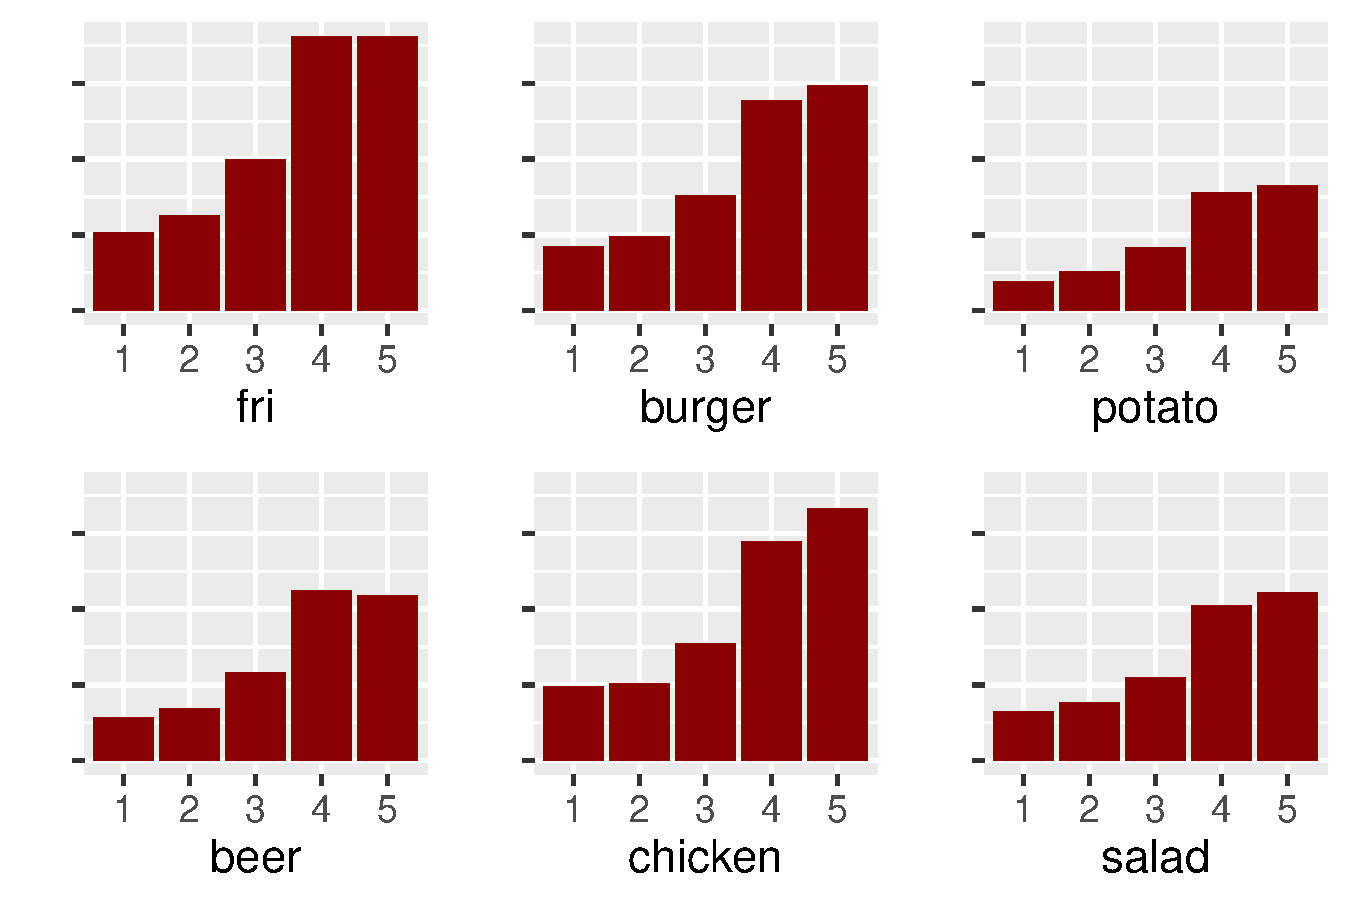
\includegraphics[width=4.6in]{food.pdf}
\end{figure}
\end{frame}

\begin{frame}
\frametitle{Word Clouds}
\begin{figure}
	\begin{minipage}[t]{0.5\linewidth}
		\centering
		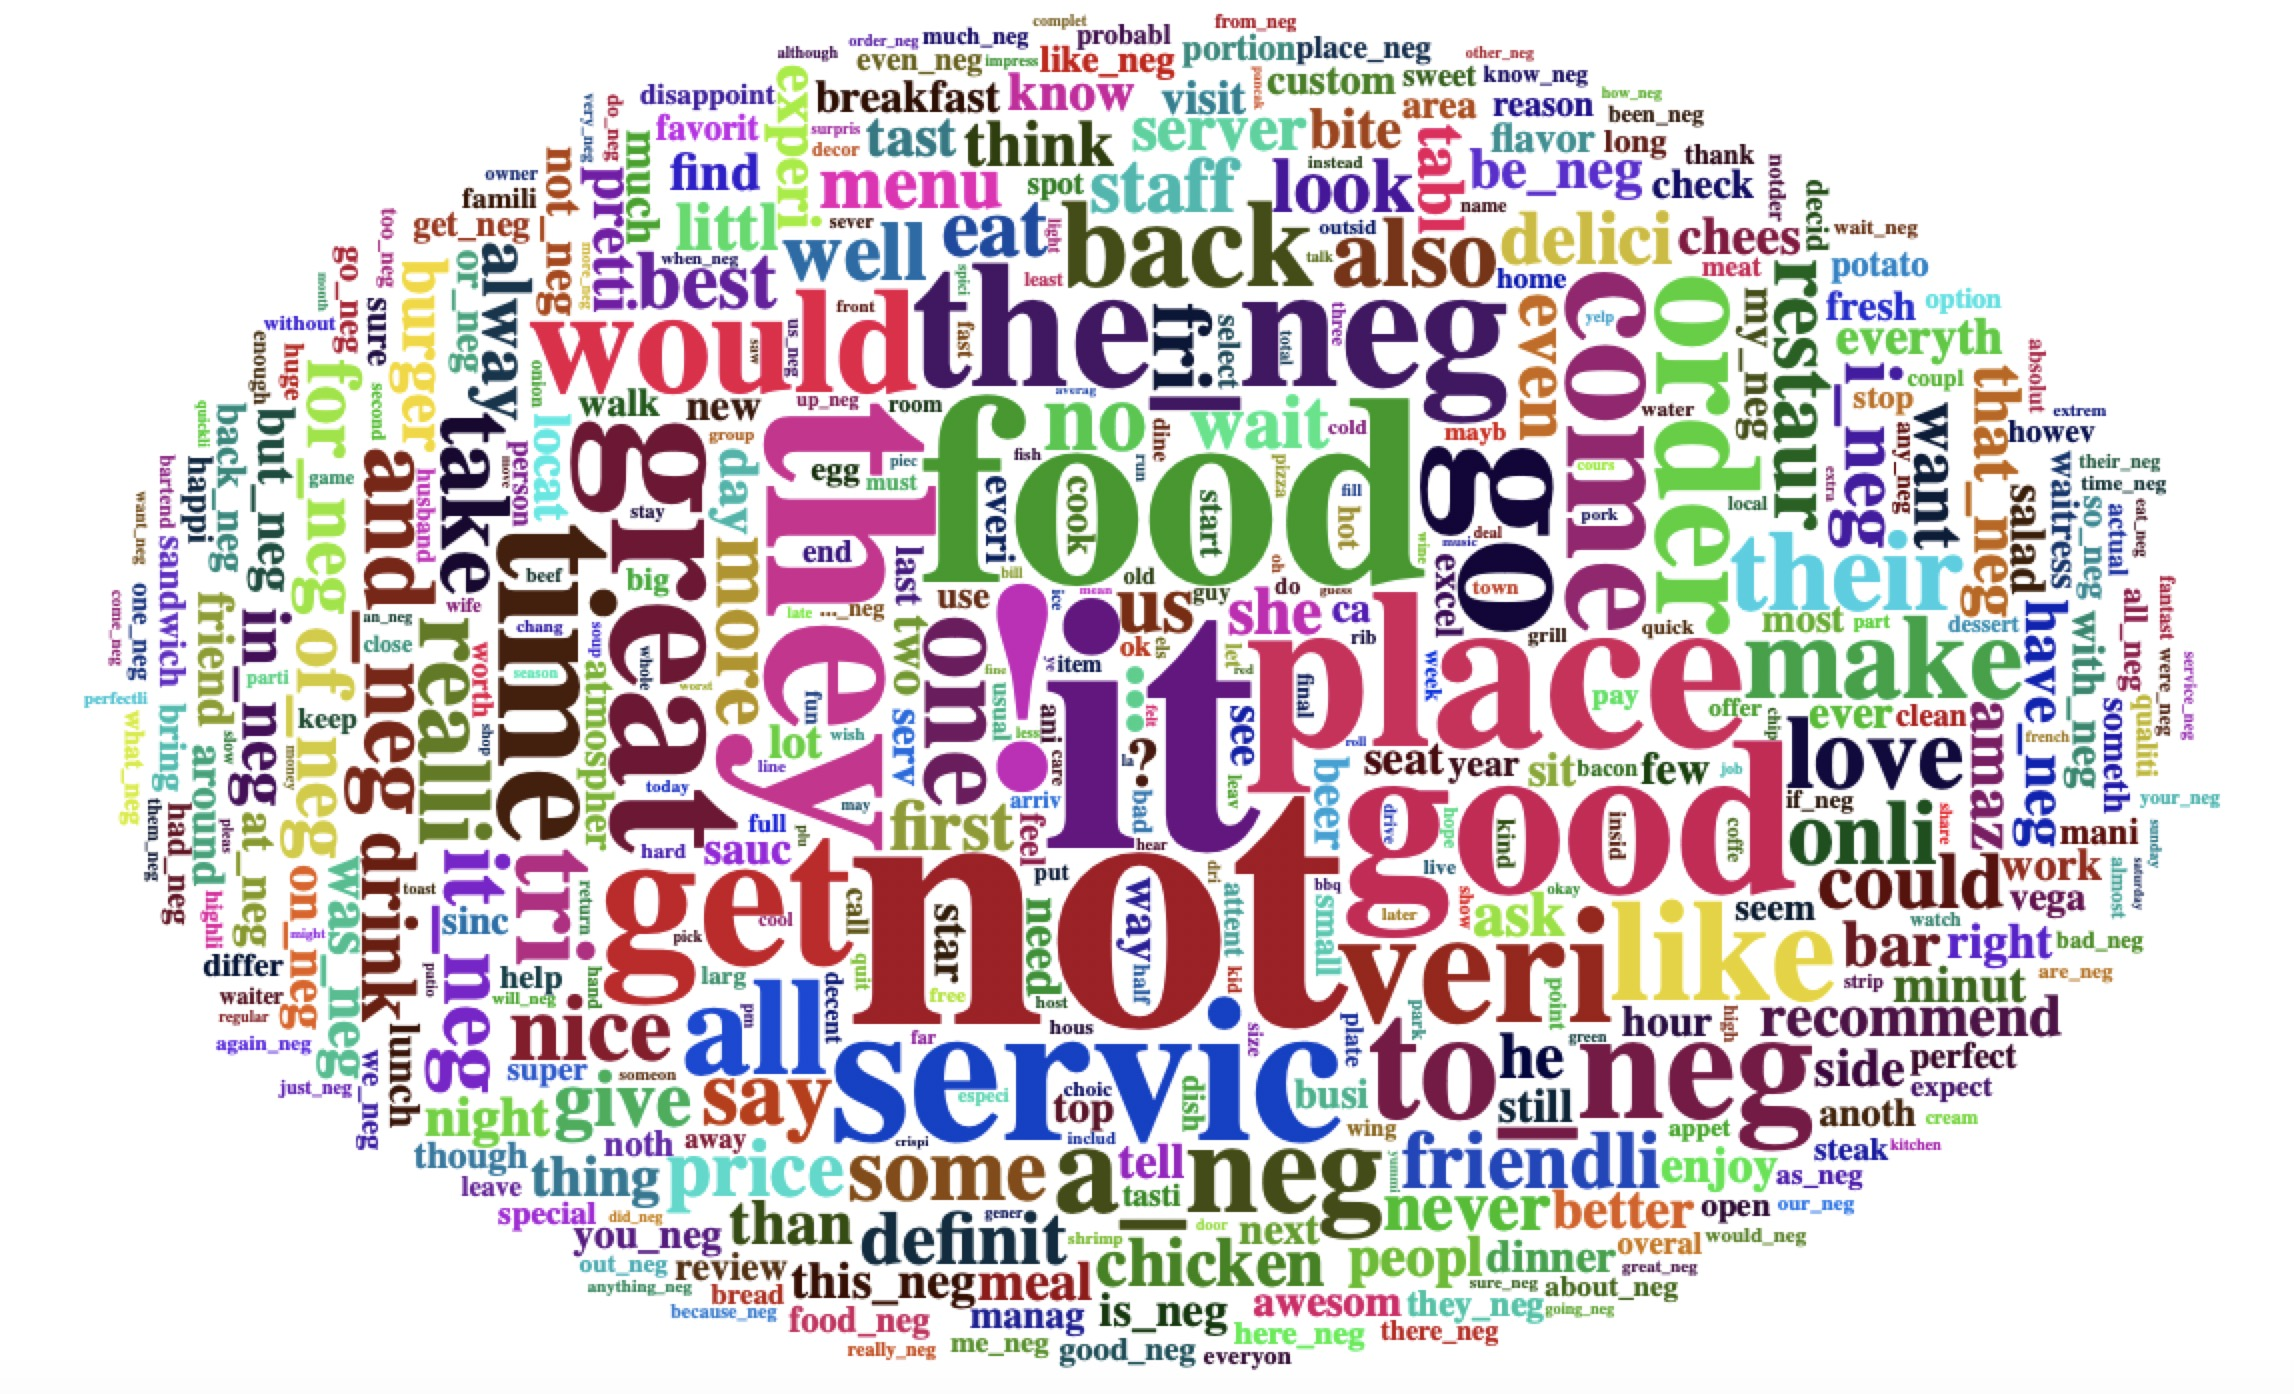
\includegraphics[width=2.2in]{all.jpg}
		\caption{Rank by Word Frequency}
		\label{fig:side:a}
	\end{minipage}%
	\begin{minipage}[t]{0.5\linewidth}
		\centering
		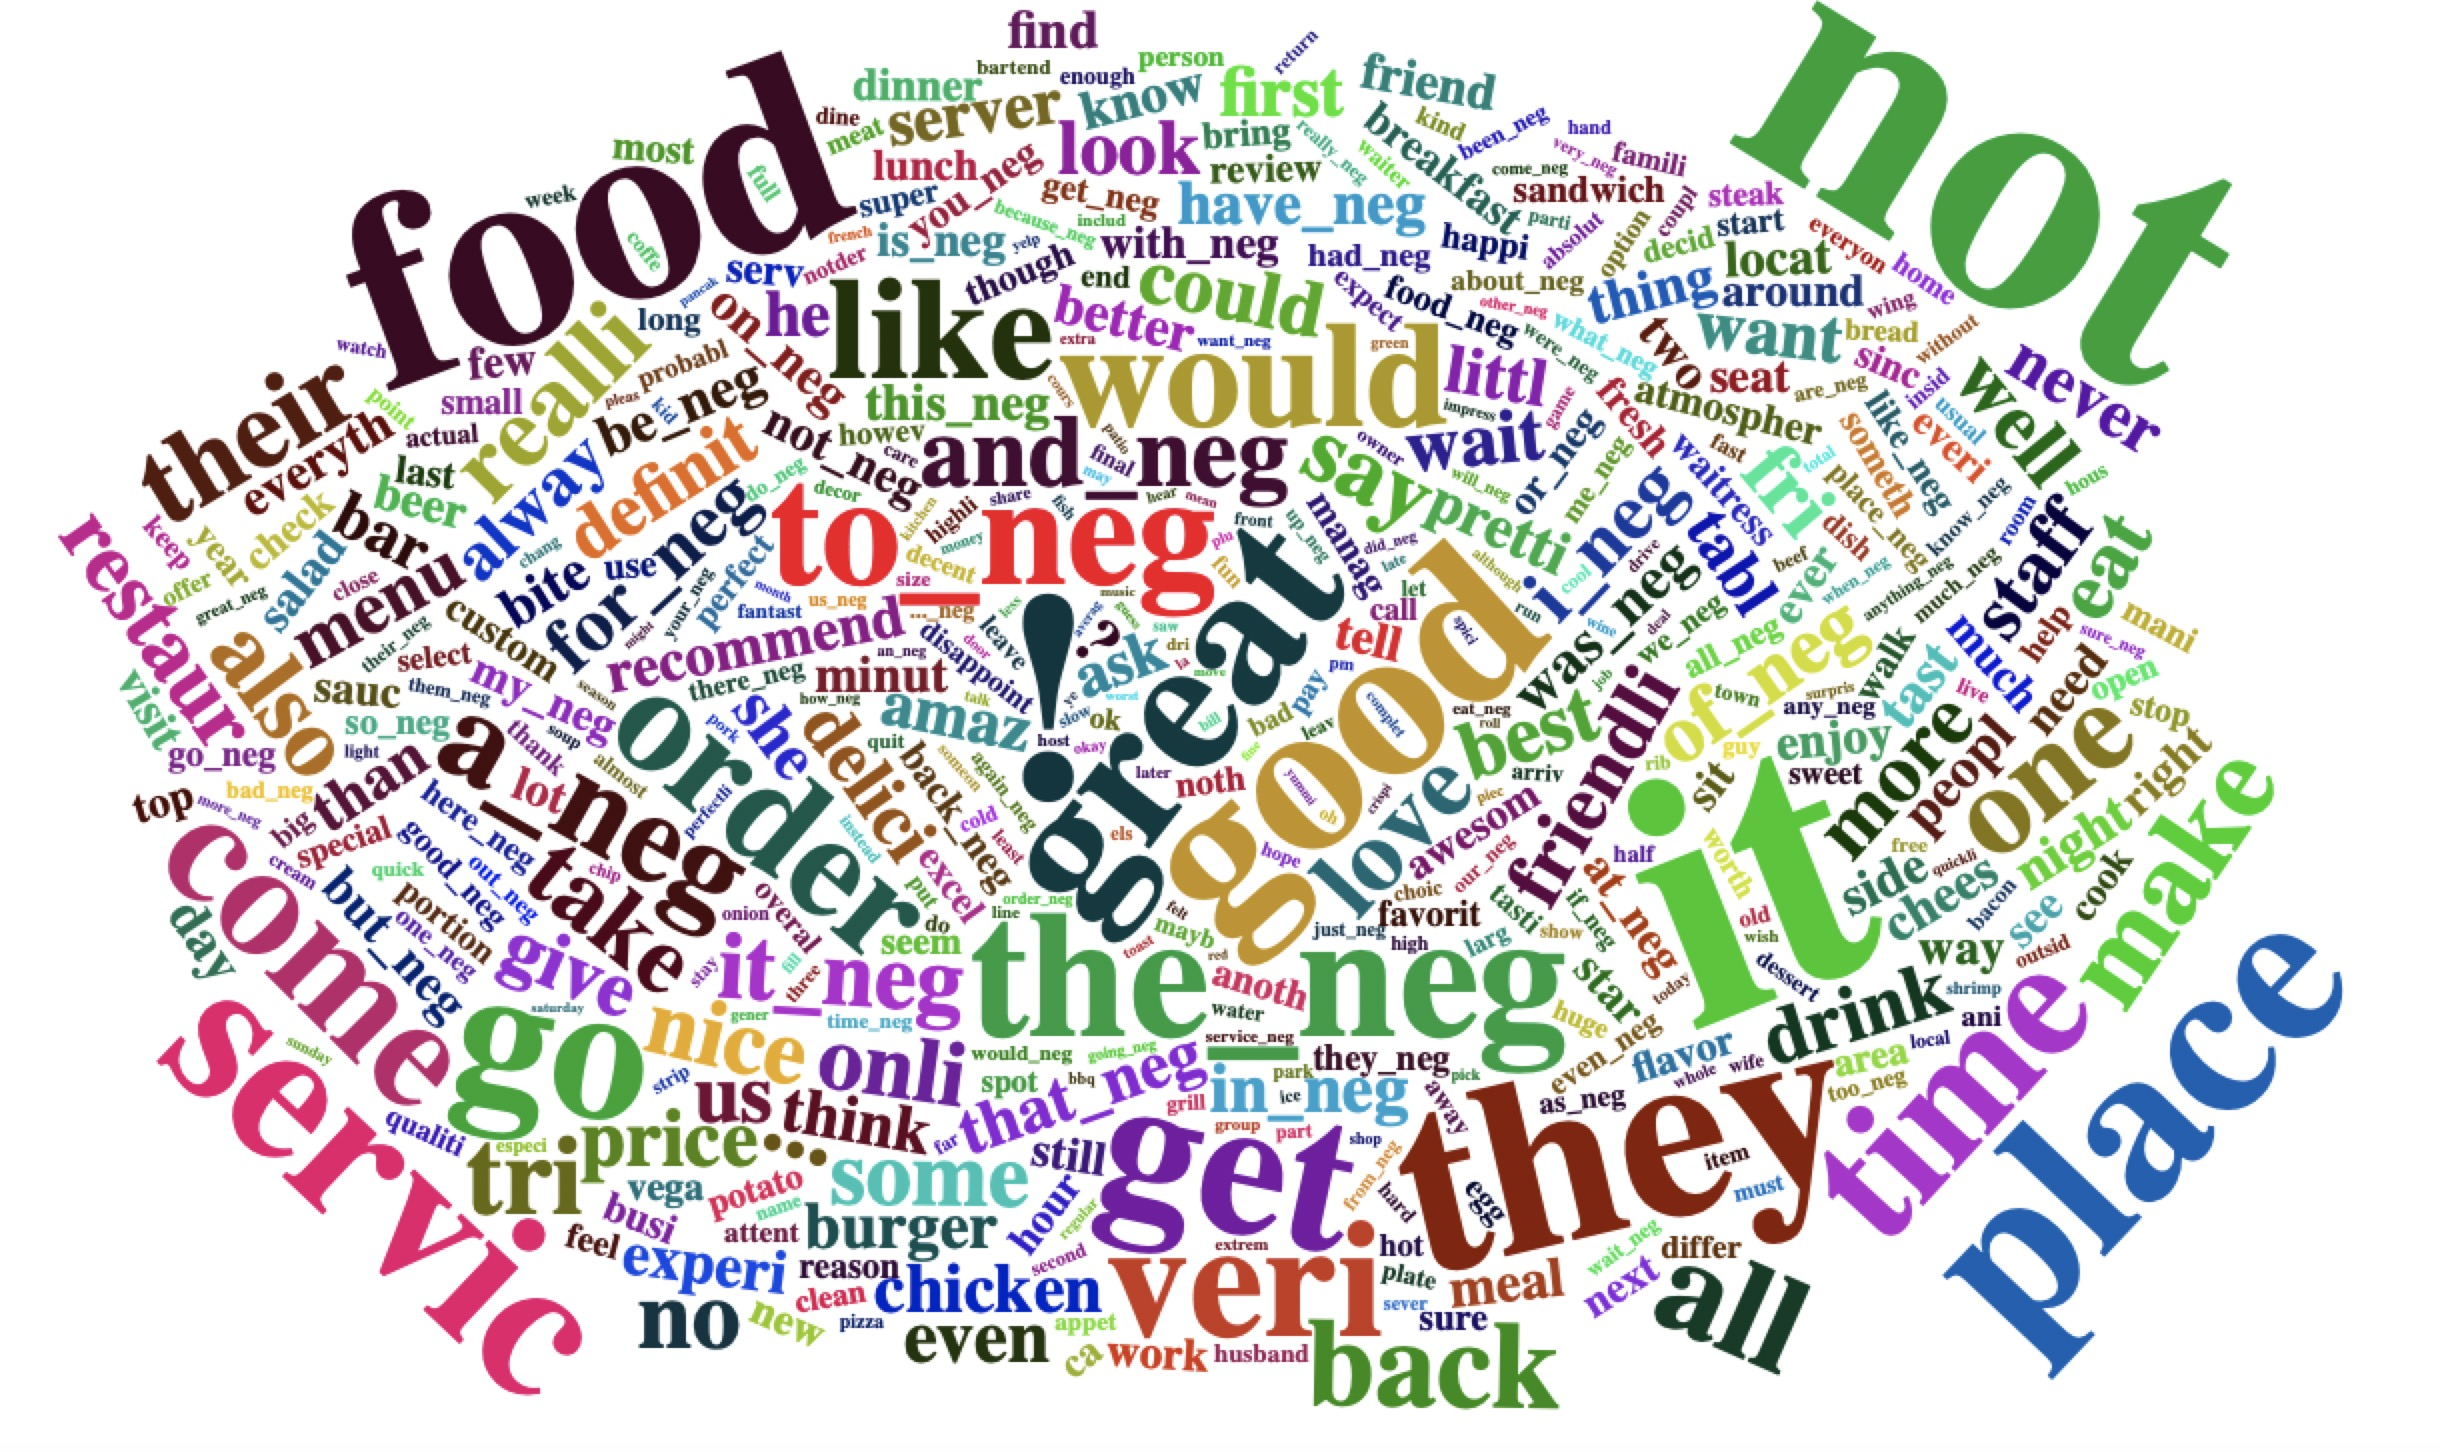
\includegraphics[width=2.2in]{info_gain.jpg}
		\caption{Rank by Information Gain}
		\label{fig:side:b}
	\end{minipage}
\end{figure}
\end{frame}

\begin{frame}
\frametitle{Traditional American Restaurants in Madison}
\begin{figure}[H]
	\centering
	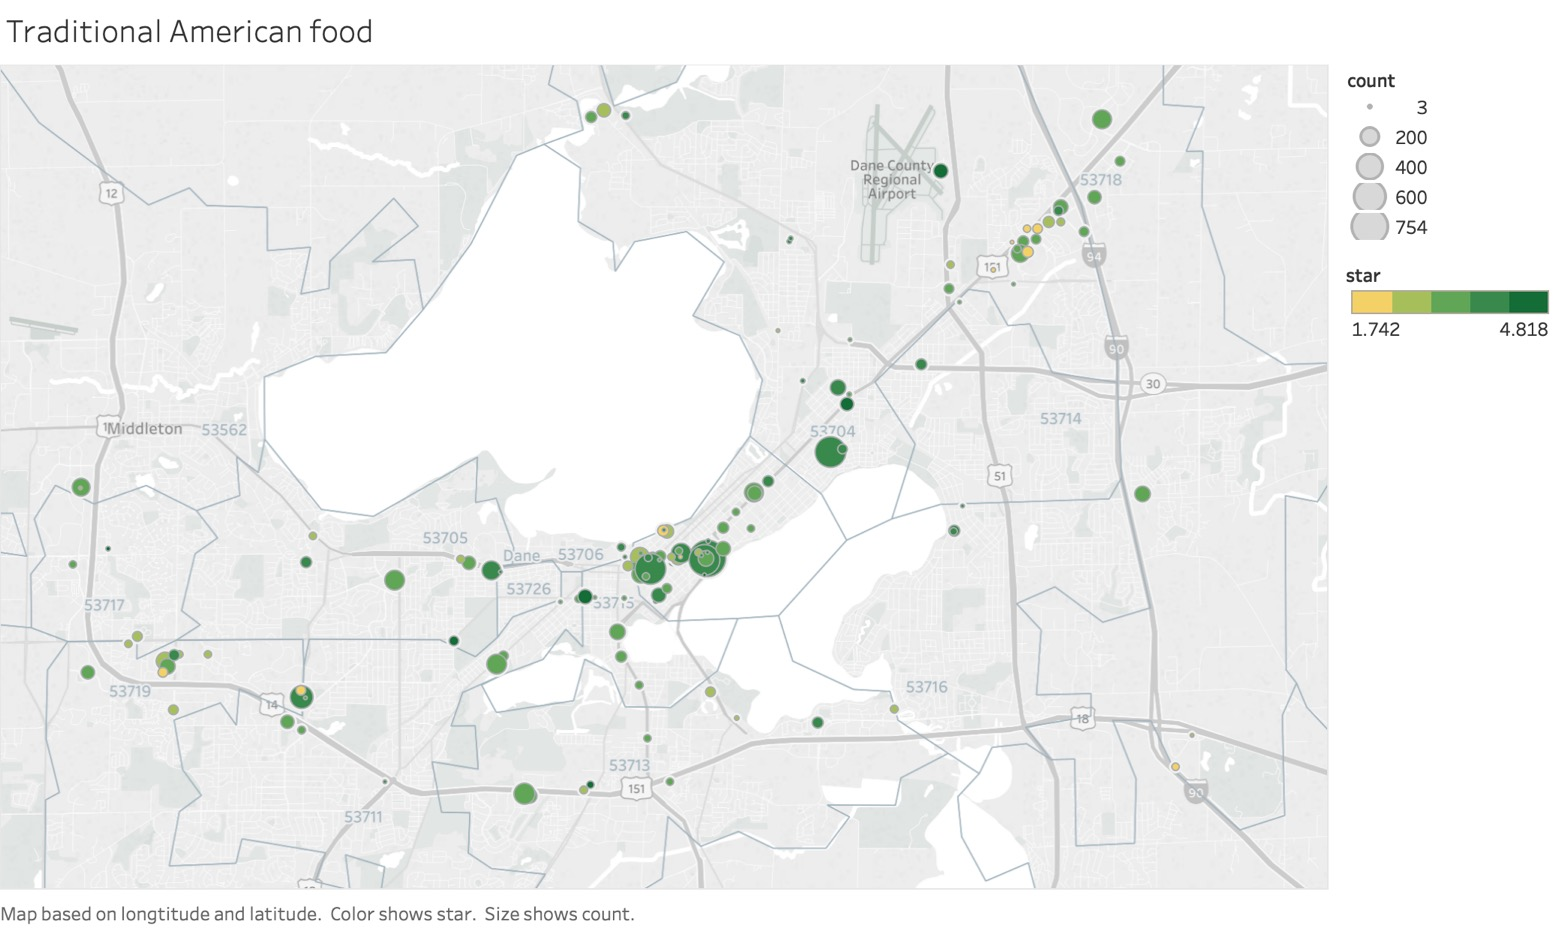
\includegraphics[width=4.6in]{american.jpg}
\end{figure}
\end{frame}

\begin{frame}
\frametitle{Chinese Restaurants in Madison}
\begin{figure}[H]
	\centering
	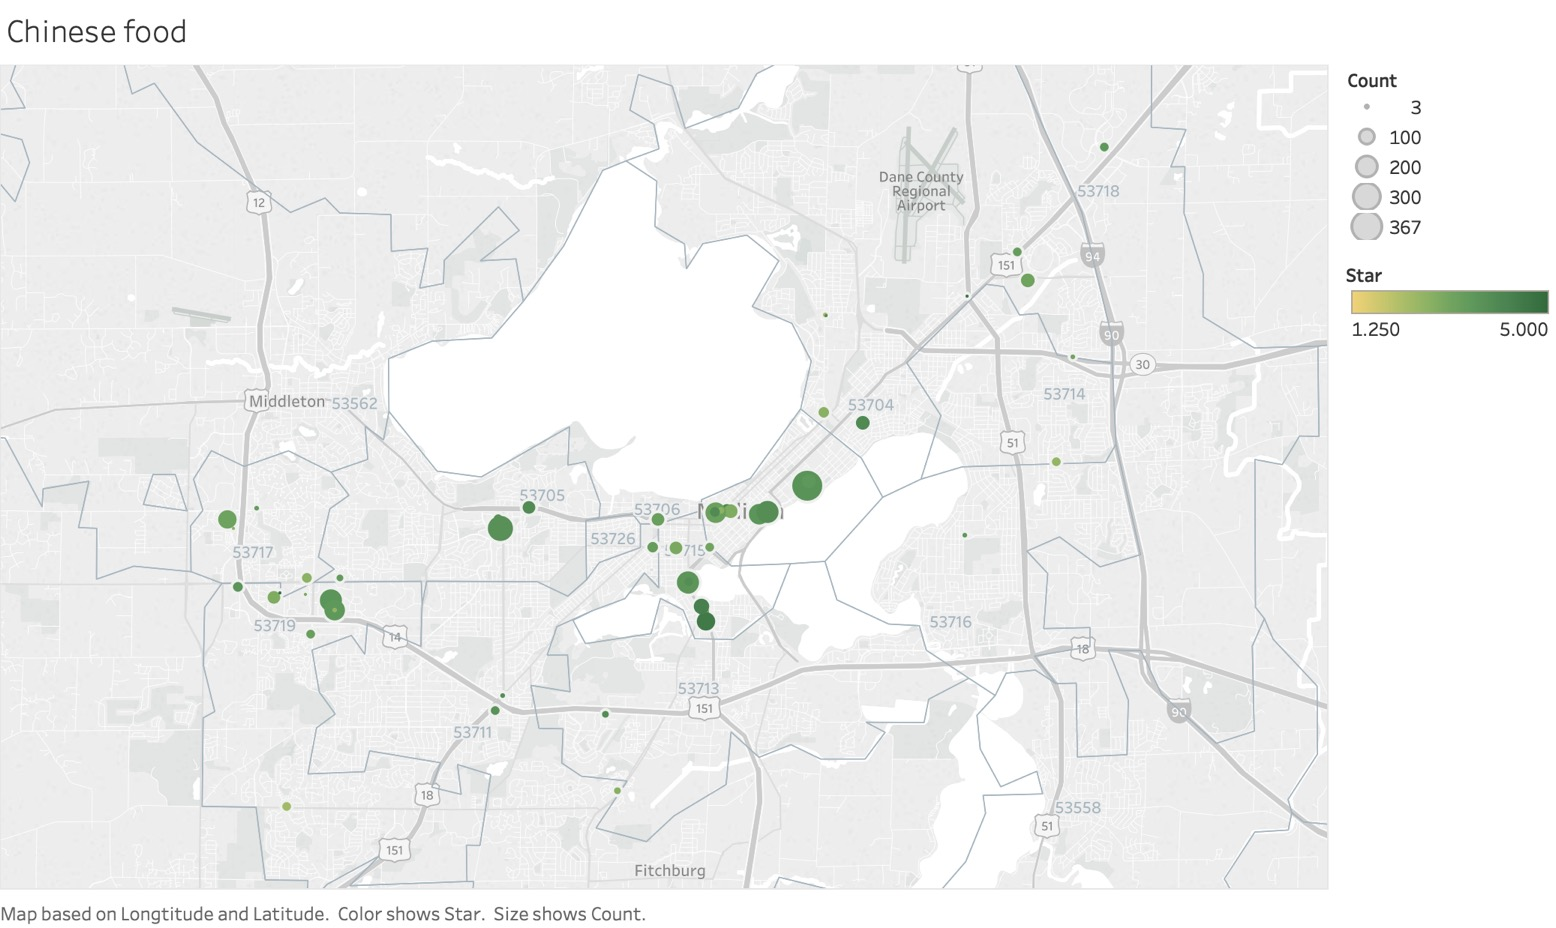
\includegraphics[width=4.6in]{chinese.jpg}
\end{figure}
\end{frame}

\begin{frame}
\frametitle{Future Work}
\begin{itemize}
	\item[\textcolor{darkred}{\textbullet}] Keep more words in final dictionary and give more specific suggestions for traditional American restaurants.
		\vspace{2ex}
	\item[\textcolor{darkred}{\textbullet}] Analyze tha data of more countries' restaurants and give some generalized suggestions.
		\vspace{2ex}
	\item[\textcolor{darkred}{\textbullet}] Star prediction: Linear regression, SVM, Bayes net etc.
	
\end{itemize}

\end{frame}

\begin{frame}
\begin{figure}[H]
	\centering
	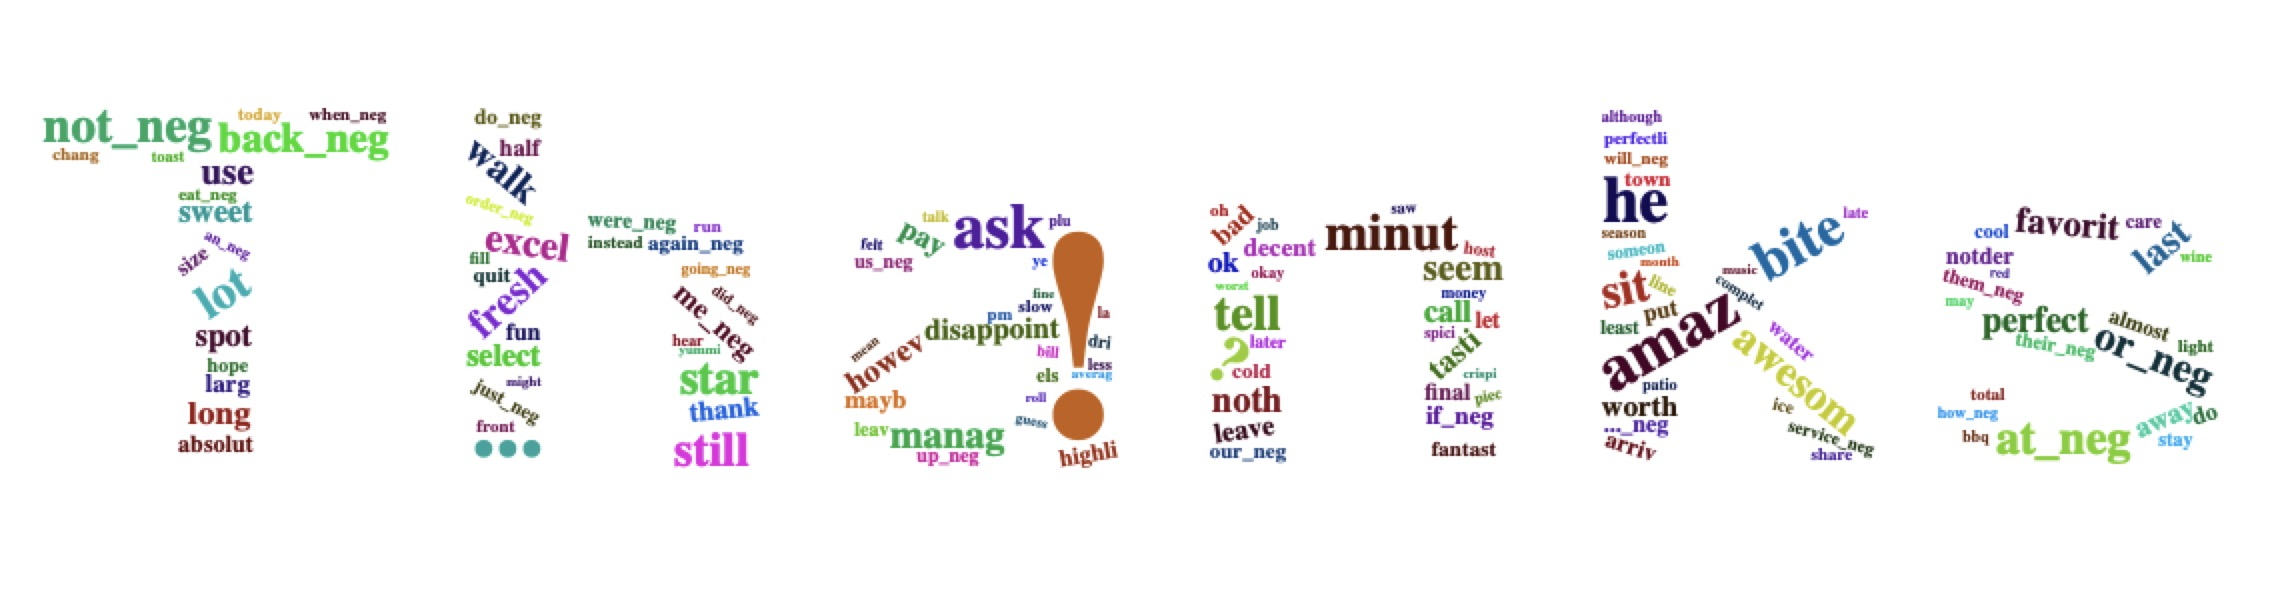
\includegraphics[width=4.6in]{thanks.jpg}
\end{figure}
\end{frame}
\end{document}